\section{Uploading images from phone}

Issue 135 was to implement a feature allowing users to upload pictures from their phone/tablet to the pictogram database. The feature description was: "As a guardian, I would like a way to add pictograms by choosing an image from my phone gallery so that I can quickly improvise if the system does not have the activity I want."
Initially, we expected the feature to require a new screen and a new \gls{bloc} for handling communication with the api. We started out by designing the view since the view should contain as little logic as possible, the \gls{ui} should not have any influence on how the logic will be implemented. The \gls{ui} also served as a skeleton to implement and test the functionality while developing. The final screen can be seen in \autoref{fig:uploadScreen}.

\begin{figure}[!ht]
  \centering
  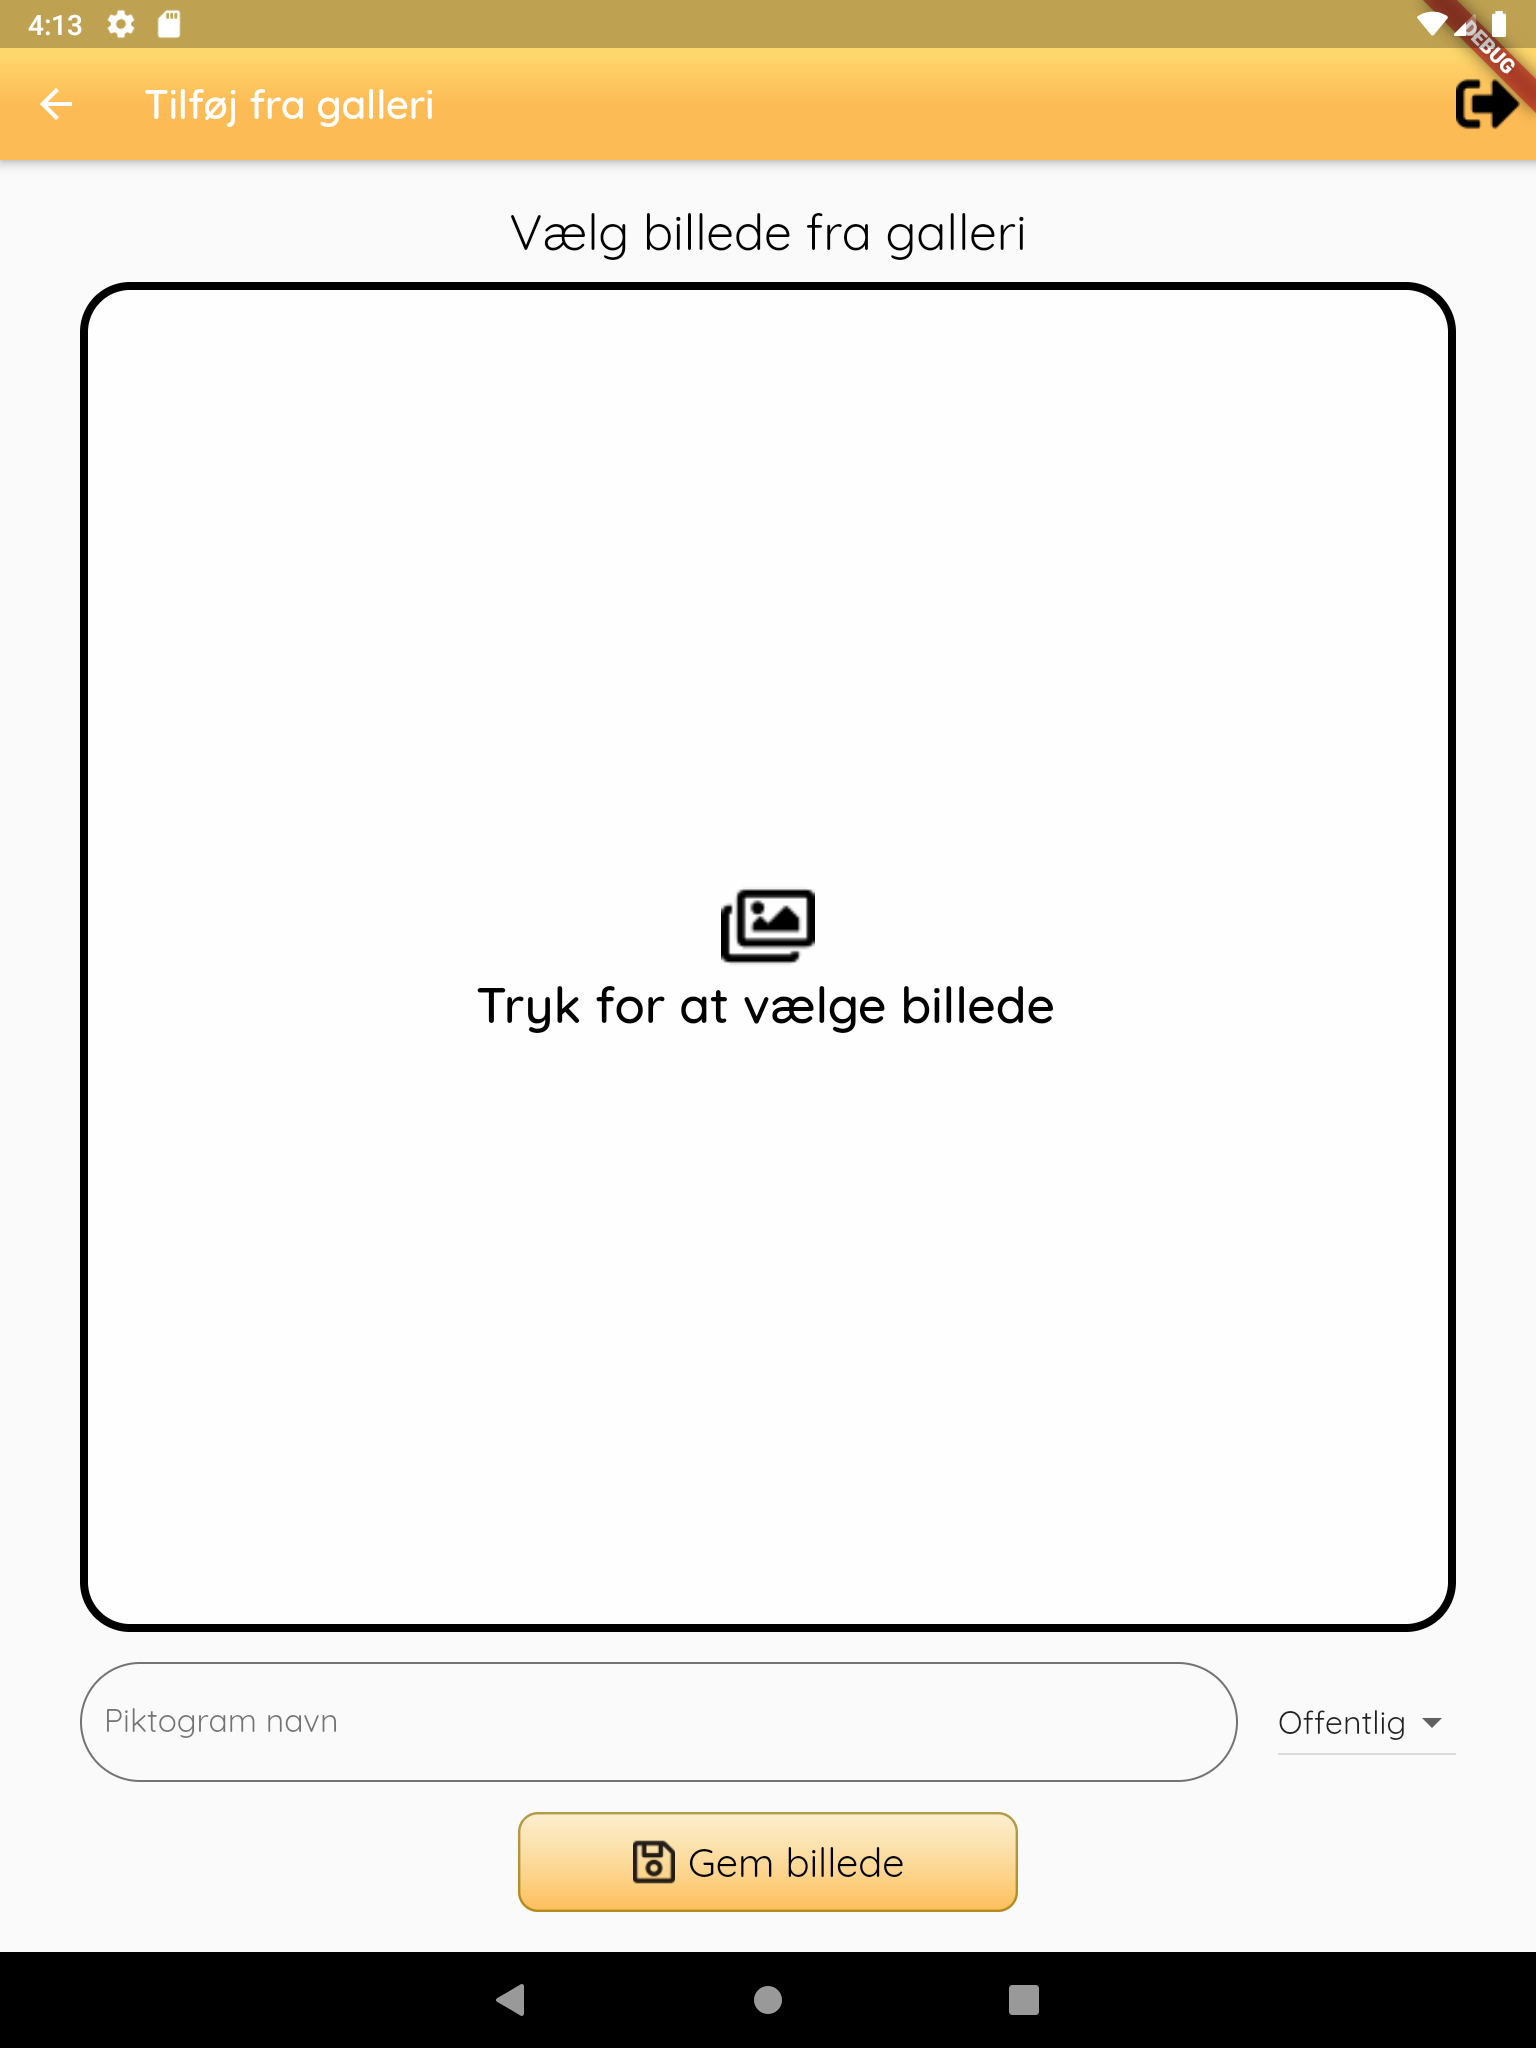
\includegraphics[width=0.7\textwidth]{figures/uploadPictogramScreen.png}
  \caption{Screenshot of the final implementation of the upload image screen}
  \label{fig:uploadScreen}
\end{figure}

We used a plugin called \textit{image\_picker} to get images from the phone.
We ran into problems with the image upload to the database, both in the \gls{fapi}, where an endpoint was not fully implemented, and in the backend \gls{api} where there was some inconsistency between the specification and implementation of the endpoint we needed. 

The \gls{fapi} issue was mitigated without any problems, but the backend \gls{api} had a flaw in the way it was configured. The endpoint for receiving an image required an image that was in either png or in jpg format. But the logic for processing the image was made expecting the image to be in a byte array format. We tested and found that it was not possible to send the image as both a file with a filetype and a byte array, the endpoint would either reject the request or throw an exception due to the data not being a byte array.
We changed the endpoint for receiving an image to not require a specific file format, which allowed us to send the image from the application to the backend.

We also wanted to make the picture uploading process more robust, as currently if e.g the server crashed when receiving the image, it would leave a corrupt file. We added a layer of protection working when both creating a new image or editing an existing one.

To make the upload process a bit more robust we introduced a four-step procedure; firstly convert the byte array to an image file with the postfix "\_temp", secondly check if there already exists an image for the given pictogram resource, if yes postfix that image whit "\_old", thirdly rename the "\_temp" image to the correct filename and lastly delete the "\_old" image if it exists.

This four-step procedure ensured that if anything went wrong in the process of the new image, it would always be possible to revert back to the old image.

Testing the implementation on a locally hosted backend server worked perfectly, but since the production environment is a bit different than the local environment we wanted to assert that it would actually work on the production environment before committing the solution.

We tested the implementation with the help of the server meta group. They created a copy of the production environment to test on. 

The implementation did not work, and we spend many hours figuring out why it worked locally but not in the production enviroment. We realized that there were an issue between docker and dotnet core's \textit{System.IO.File.Move} function. The issue is that dotnet core's low-level implementations of \textit{System.IO.File.Move} uses a hard-link, which is not supported by docker due to some security measures. We researched the issue and found that this was known to the dotnet core maintainers, but they do not intend to fix it as of the time of writing.

We attempted many different work arounds to mitigate the issue between docker and dotnet core, but nothing worked. In the end, we came to the conclusion that either we leave this as an openw issue for next years students or we remove the extra robustness of the upload and write the byte array directly to the file. The latter was an option since that would not include any \textit{System.IO.File.Move} commands. After consulting with \gls{POT} it was decided that we would implement it without the additional robustness.

The activity of debugging the upload issues also produced other important updates to the architecture. We discovered that all the  deployed backend enviroments (production, development, and testing ) used the same file storage for pictograms. This meant that when testing the file upload we affected the data for production and development directly. The server group fixed this issue and ensured that every deployed backend has its own file storage for pictograms. Another discovery was that the production and development deployments used the same database. This was also fixed.

In the end, the feature was implemented successfully, with the compromise that if something goes wrong in the upload process a corrupt file can be introduced into the system.
